\documentclass{scrbook} % <= Druckversion: "scrbook" / Bildschirmversion: "scrreprt"
\usepackage[english,bibtex]{osm-thesis} % <= Sprache der Arbeit ("ngerman"/"english"), Biblatex-Backend ("bibtex"/"biber")
\usepackage{cleveref}
\usepackage{acro}
\usepackage{CJKutf8}
\usepackage{listings}



\graphicspath{{images}}



% ABOUT
\newcommand{\hpitype}{Bachelor's thesis}
\newcommand{\hpiauthor}{Lina Wilske}
\newcommand{\hpititle}{Machine Learning-based User Movement Prediction in Layer 2 Networks}
\newcommand{\hpititleother}{Vorhersage von Benutzerbewegungen in Layer 2 Netzwerken basierend auf Maschinellem Lernen} % <= das Studienreferat verlangt einen deutschen UND englischen Titel
\newcommand{\hpisupervisor}{Prof.\,Dr.\,Holger Karl \\ Leonard Paeleke}
\newcommand{\hpichair}{Internet Technology and Softwarization Group}
\newcommand{\hpidate}{\today}

% Acronyms before everything else
\DeclareAcronym{ap}{
    short=AP,
    long=Access Point
}
\DeclareAcronym{rssi}{
    short=RSSI,
    long=Received Signal Strength Indication
}
\DeclareAcronym{bssid}{
    short=BSSID,
    long=Basic Service Set Identifier
}
\DeclareAcronym{ssid}{
    short=SSID,
    long=Service Set Identifier
}
\DeclareAcronym{mac}{
    short=MAC,
    long=Media Access Control
}
\DeclareAcronym{wifi}{
    short=Wi-Fi,
    long=Wireless Fidelity
}
\DeclareAcronym{ssf}{
    short=SSF,
    long=Signal Strength Factor
}
\DeclareAcronym{llf}{
    short=LLF,
    long=Link Loss Factor
}
\DeclareAcronym{ml}{
    short=ML,
    long=Machine Learning
}
\DeclareAcronym{rnn}{
    short=RNN,
    long=Recurrent Neural Network
}
\DeclareAcronym{lstm}{
    short=LSTM,
    long=Long Short-Term Memory
}
\DeclareAcronym{gru}{
    short=GRU,
    long=Gated Recurrent Unit
}
\DeclareAcronym{arima}{
    short=ARIMA,
    long=Autoregressive Integrated Moving Average
}
\DeclareAcronym{mlp}{
    short=MLP,
    long=Multilayer Perceptron
}
\DeclareAcronym{mse}{
    short=MSE,
    long=Mean Squared Error
}
\DeclareAcronym{mae}{
    short=MAE,
    long=Mean Absolute Error
}
\DeclareAcronym{uuid}{
    short=UUID,
    long=Universally Unique Identifier
}
\DeclareAcronym{TxPower}{
    short=TxPower,
    long=Transmission Power
}
\DeclareAcronym{MajorID}{
    short=MajorID,
    long=Major Identifier
}
\DeclareAcronym{MinorID}{
    short=MinorID,
    long=Minor Identifier
}
\DeclareAcronym{ai}{
    short=AI,
    long=Artificial Intelligence
}
\DeclareAcronym{TCP}{
    short=TCP,
    long=Transmission Control Protocol
}
\DeclareAcronym{wlan}{
    short=WLAN,
    long=Wireless Local Area Network
}
\DeclareAcronym{tsc}{
    short=TSC,
    long=Time Series Classification
}
\DeclareAcronym{hmm}{
    short=HMM,
    long=Hidden Markov Model
}
\DeclareAcronym{relu}{
    short=ReLU,
    long=Rectified Linear Unit
}

% DOCUMENT
\bibliography{bibliography}



\begin{document}

	
	% Einband
	\pagenumbering{alph}
	%\ifisbook\begin{titlepage}
	\setlength{\evensidemargin}{0.5\evensidemargin+0.5\oddsidemargin}
	\setlength{\oddsidemargin}{\evensidemargin}

	\centering

	\raisebox{-0.5\height}{
\includegraphics[width=5.5cm]{images/hpi_logo_black.pdf}}
	\hspace*{.2\textwidth}
	\raisebox{-0.5\height}{
\includegraphics[width=4cm]{images/uni_logo_black.pdf}}
	
	\vspace*{4\baselineskip}
	{\usekomafont{subject}\hpitype}\par
	
	\vfill
	{\usekomafont{title}\hpititle\par}
	\vspace*{\baselineskip}
	{\usekomafont{subtitle}\hpititleother}\par
	
	\vfill
	{\textbf{\phantom{\iflanguage{ngerman}{von}{by}}} \\
	 \smallskip\usekomafont{author}\hpiauthor}\par
	
	\vfill
	\phantom{\begin{minipage}{\textwidth}
	{\textbf{\iflanguage{ngerman}{Betreuung}{Supervisors}}\\
	\usekomafont{publishers}\smallskip\hpisupervisor\\ \textit{\hpichair}\\}
	\end{minipage}}
	
	\vfill
	{\usekomafont{date}\iflanguage{ngerman}{Hasso-Plattner-Institut an der Universität Potsdam}{Hasso Plattner Institute at University of Potsdam}}\par
	\vspace*{\baselineskip}
	{\usekomafont{date}\hpidate}\par
	
\end{titlepage}\fi
	\ifisbook\cleardoubleemptypage\fi
	
	% (Haupt-)Titelseite, Abstract, ggf. Danksagung & Inhaltsverzeichnis
	\pagenumbering{roman}
	\begin{titlepage}
	\centering

	\raisebox{-0.5\height}{
\includegraphics[width=5.5cm]{images/hpi_logo_srgb.pdf}}
	\hspace*{.2\textwidth}
	\raisebox{-0.5\height}{
\includegraphics[width=4cm]{images/uni_logo_srgb.pdf}}

	\vspace*{4\baselineskip}
	{\usekomafont{subject}\hpitype}\par
	
	\vfill
	{\usekomafont{title}\hpititle\par}
	\vspace*{\baselineskip}
%	{\usekomafont{subtitle}\hpititleother}\par
	
	\vfill
	{\textbf{\iflanguage{ngerman}{von}{by}}\\ 
		\smallskip\usekomafont{author}\hpiauthor}\par
	
	\vfill
	{\textbf{\iflanguage{ngerman}{Betreuung}{Supervisors}}\\ 
		\usekomafont{publishers}\smallskip\hpisupervisor\\ \textit{\hpichair}\\}
	
	\vfill
	{\usekomafont{date}\iflanguage{ngerman}{Hasso-Plattner-Institut an der Universität Potsdam}{Hasso Plattner Institute at University of Potsdam}}\par
	\vspace*{\baselineskip}
	{\usekomafont{date}\hpidate}\par

	\setcounter{page}{1}

\end{titlepage}


	\ifisbook\cleardoubleemptypage\fi% => Wenn die Arbeit auf Deutsch verfasst wurde, verlangt das Studienreferat KEINEN englischen Abstract

% englischer Abstract
\null\vfil
\begin{otherlanguage}{english}
\begin{center}\textsf{\textbf{\abstractname}}\end{center}

\noindent ...

\end{otherlanguage}
\vfil\null





	%\ifisbook\cleardoubleemptypage\fi\vspace*{\fill}
\begin{center}\textsf{\textbf{Dedication}}\end{center}

\noindent ...

\vspace*{\fill}
	\tableofcontents
	\cleardoublepage

	% Textteil
	\pagenumbering{arabic}
	\chapter{Introduction}\label{sec:intro}

% Darstellung des Themas der Arbeit
% genaue Auflistung der Fragestellungen (wieso Thema relevant?)
% knapper Überblick über Schritte der Problembehandlung:

% - Hinführung Thema
% - Herleitung und Ausformulierung der Fragestellung
% - Abgrenzung des Themas (Angabe von Aspekten, die zum Thema gehören, aber nicht behandelt/ausgeklammert werden)
% - Aufbau der Arbeit (Begründung der Gliederung)


In large-scale \ac{wifi} environments such as office buildings, shopping malls, and airports, where multiple \acp{ap} are required, people often move around indoors with their mobile devices.
To maintain a stable connection to the \ac{ssid} a device connects to, it must remain in the range of the \ac{ap} or may roam to another \ac{ap} with the same \ac{ssid}.
Roaming has been an essential feature of \ac{wifi} since the advent of the 802.11k\cite{802.11k} feature.
This process improved with \ac{ap}-initiated roaming, introduced in 802.11r\cite{802.11r}.
However, the current roaming process does not account for human movement patterns. 
For example, if a station is moving away from \ac{ap}1 towards \ac{ap}2, ideally, \ac{ap}2 should initiate the roaming process.
Furthermore, an AP may instruct a client device to roam based on signal strength without considering the device's trajectory or the user's likely destination.
The existing solutions need to be more robust and often lead to frequent hand-offs, inefficient resource usage, and in some cases, dropped connections.
This thesis will explore using time series \ac{ml} model to predict the top 3 \acp{bssid} a station may connect to next.
Therefore, this thesis needs data with \ac{wifi}, waypoint of clients and sensor data, e.g. acceleration.

A time series \ac{ml} models require time series data as input.
There are two possible data sources: generate new or utilize existing data. 
Data generation needs a comprehensive plan for accounting data setup and collection.
The generation is a time-consuming process and needs a lot of planning and evaluation beforehand.
Therefore, this thesis will utilize pre-existing data from a 2021 competition by Microsoft Research\cite{IndoorLocationNavigation}.
The data will be analyzed to determine what specific parts of the data we will use for the \ac{ml} model.

Furthermore, the data will be prepared for a time series \ac{ml} model.
After that, we will discuss the suitability of some pre-selected \ac{ml} models for the task. 
Due to the large number of data, this thesis will implement improving it, and evaluate the model's performance for a specific site and floor.

%\noindent
	\chapter{Background}\label{ch:background}

The basic information in this chapter helps to comprehend the key ideas covered in this thesis.
The field of \ac{ml} is extensive, with many models created for diverse tasks, each with advantages and uses.
This chapter will provide a brief overview of the models discussed and used in this thesis, as well as the concepts of time series prediction and hyperparameter tuning.

\section{Classification}

Classification models in \ac{ml} are designed to categorize input data into specific classes using input features and labels.
In supervised learning, models are trained with input vectors and their associated target vectors, which represent the desired output or correct category for each input.
Classification problems, such as digit recognition, assign input vectors to discrete categories.
Practical applications include determining whether an email is spam or a fraudulent transaction \cite{binary-classification}.
Multi-class classification, a set of classification, differentiates among more than two classes \cite{BishopPatternRecognition}.
In this thesis, a multi-class classification model will be used to predict which \ac{ap} a user will be closest to, based on the \ac{rssi} from the \acp{ap} and the user's trajectory.


\section{Univariate and Multivariate Time Series}

A time series is univariate if one observation is recorded sequentially over time, e.g., temperature or stock prices.
If another observation was recorded over time together with the temperature, such as humidity, then the time series is multivariate \cite{brownleeDeepLearningTime}.

\section{Time Series Prediction}

Time series prediction involves training models on sequences of observations to predict the next value in the sequence \cite{brownleeDeepLearningTime}.
These sequences, consisting of chronologically arranged data points, are prevalent in numerous domains, including stock prices.
Due to the inherent temporal dependencies in time series data, where subsequent data points influence previous ones, specific machine learning techniques are applied.
These techniques aim to capture and leverage temporal patterns within the data, predicting future trends based on historical observations \cite{neptune-ai}.

%\fmhkn{this is not structured so nicely. We are mixing problems -- time-series prediction -- with techniques -- MLP -- and mathematicl structures -- HMM. I am confused :-/ }

\section{Machine Learning Models for Time Series Prediction}

In machine learning research, time series prediction has attracted great interest.
As a result, numerous machine learning models designed specifically to handle sequential data have been created.
While some of these models are based on older established statistical techniques, others find their inspiration in more recent developments.
This section gives a summary of a few models that are important to this thesis.

\subsection{Hidden Markov Model}

\ac{hmm} is a statistical model that assumes the system being modeled is a Markov process with unobserved states \cite{hmm-rabiner-1989}.
\acp{hmm} are mainly known for their application in temporal pattern recognition, such as speech and handwriting.
They describe the probability of a sequence of observable data, which is assumed to result from a sequence of hidden states, each producing an observable output according to a particular probability distribution.

\subsection{Multilayer Perceptron}

\ac{mlp}, also known as a feedforward artificial neural network, is a class of deep learning models primarily used for supervised learning tasks \cite{mlp-backpropagation-rumelhart}.
An MLP consists of multiple layers of nodes in a directed graph, each fully connected to the next one.
Each node in one layer is connected with certain weights to every node in the following layer.
\acp{mlp} apply a series of transformations, typically nonlinear, to the input data using activation functions, such as the sigmoid or \ac{relu}, facilitating the model's ability to model complex patterns and dependencies in the data \cite{goodfellow_deep_2016}.

\subsection{Recurrent Neural Networks}

\ac{rnn} is a neural network well-suited to sequential data because of its design \cite{hopfield-rnn}.
Unsuch as traditional feedforward neural networks, an \ac{rnn} possesses loops in its topology, allowing information to persist over time.
This unique characteristic enables the model to use its internal state (memory) to process sequences of inputs, making it ideally suited for tasks involving sequential data such as speech recognition, language modeling, and time series prediction \cite{elman_finding_1990}.

\subsubsection{Long Short-Term Memory}

\ac{lstm} is a special kind of RNN, capable of learning long-term dependencies \cite{lstm-hochreiter}.
\acp{lstm} were designed to combat the ``vanishing gradient'' problem in traditional \acp{rnn}. 
This problem made it difficult for other neural networks to learn from data where relevant events occurred with significant gaps between them.
The key to the ability of the \acp{lstm} is its cell state and the accompanying gates (input, forget, and output gate), which regulate the flow of information in the network.

\section{Hyperparameter tuning}\label{sec:hyperparameter-tuning}

In \ac{ml}, hyperparameters play an important role in model development as they may improve the model's performance \cite{yuHyperParameterOptimizationReview2020}.
These are parameters such as the learning rate, neural network layers, and the number of windows or batch sizes.
Proper selection of hyperparameters, known as hyperparameter tuning or optimization, is crucial to optimize model performance.
This iterative procedure involves exploring various hyperparameter combinations for the configuration that yields the most accurate predictions.
Hyperparameters can be tuned by, e.g., random search, which can be done manually or using libraries.
This thesis will use keras-tuner \footnote{Keras-tuner, the hyperparameter optimization framework for keras: \url{https://github.com/keras-team/keras-tuner}} to tune the hyperparameters of the \ac{lstm} model.
\texttt{RandomSearch} is a hyperparameter optimization algorithm that randomly searches the hyperparameter space for the best configuration.
The user predefines the hyperparameter space, and the algorithm tries out different hyperparameters in this space.

	\chapter{Dataset analysis and preparation}\label{ch:data-ana}

As mentioned in \Cref{ch:intro}, the dataset used in this thesis is the Indoor Location \& Navigation from kaggle, which was part of a competition of Microsoft Research in 2021 \cite{IndoorLocationNavigation}.
The company ``\(XYZ^{10}\)''\footnote{Website of \(XYZ^{10}\): https://dangwu.io} recorded the data in shopping malls and was provided by Microsoft Research for this competition.
The goal of the competition was to predict the indoor position of users' smartphones based on real-time sensor data and user trace data.
The prediction for this competition contain the floor and waypoint at a certain timestamp.
However, this thesis will not predict the floor and waypoint but the next \ac{bssid} a device may connect to based on the \ac{rssi} of the \acp{ap} and the trajectory of the user, as this prediction is more useful for the roaming process.
Therefore, the dataset will be analyzed to determine what parts of the data I use for the \ac{ml} model.

\section{Components of the dataset}\label{sec:data}
As noted in the kaggle notebook ``Indoor Navigation: Complete Data Understanding'' \cite{IndoorNavigationUnderstanding} the data consists of 3 parts:

\begin{itemize}
    \item a \texttt{train} folder with train path files, organized by site and floor.
    \item a \texttt{test} folder with test path files, organized by site and floor but without waypoint data.
    \item a \texttt{metadata} folder with floor metadata, organized by site and floor, which includes floor images, further information, and a geojson map.
\end{itemize}

The train folder contains 204 subfolders representing each shopping mall (site) where the data was recorded.
In each site folder are a minimum of one and a maximum of twelve subfolders, which represent the floors of the site; the median is five floors.
Overall, there are 26,925 files, each containing the movement of a person for a specific site and floor.
Per floor, there are between one and 284 files with a median of 14.
The floor F1 of the site \begin{CJK*}{UTF8}{gbsn}银泰城(城西店)\end{CJK*} (Yintai City (Chengxi Branch)) in the train folder of the competition, has the most files.

The submission files and the test folder will not be used for this thesis.
Instead, I will generate the test set out of the train data because the goal is not to predict the floor and site name for a specific timestamp but to predict the \ac{bssid} to which a device may connect next, which is an entirely different task.
Therefore, I will not analyze the content of the test and metadata folders in detail, but further focus on the content of the train folder.


\section{File structure}\label{sec:file-structure}

Each file in each floor folder is a \textbf{.txt} file.
The first contains the start time of the recording, the second site information \texttt{SiteID} as hash, \texttt{SiteName}, \texttt{FloorId} as hash, and \texttt{FloorName}.

\lstset{
    basicstyle=\scriptsize\ttfamily,
    breaklines=true,
    escapeinside={(*@}{@*)},
    numbers=left,
    numberstyle=\tiny\color{gray},
    stepnumber=1,
    numbersep=5pt,
}

\begin{lstlisting}[caption={A snippet from the dataset of the file 5daa9e38df065a00069beb79.txt of the floor F4},label={lst:dataset}]
    #   startTime:1571462193934
    #   SiteID:5d27099303f801723c32364d SiteName:(*@\begin{CJK*}{UTF8}{gbsn}银泰百货(庆春店)\end{CJK*}@*) FloorId:5d27099303f801723c323650 FloorName:4F
    1571462193944   TYPE_WAYPOINT   57.885998   69.501526
    1571462194071   TYPE_ACCELEROMETER  -0.95254517 0.7944031   8.928757    2
    1571462194071   TYPE_MAGNETIC_FIELD -25.65918   -4.4784546  -28.201294  3
    1571462194071   TYPE_GYROSCOPE  -0.22373962 -0.07733154 -0.16847229 3
    1571462194071   TYPE_ROTATION_VECTOR    0.04186145  -0.02101801 -0.72491926 3
    1571462194071   TYPE_MAGNETIC_FIELD_UNCALIBRATED    -4.8568726  10.406494   -387.44965  20.802307   14.884949   -359.24835  3
    1571462194071   TYPE_GYROSCOPE_UNCALIBRATED -0.22218323 -0.068359375    -0.1628418  0.0026245117    9.765625E-4 -7.6293945E-4   3
    1571462194071   TYPE_ACCELEROMETER_UNCALIBRATED -0.95254517 0.7944031   8.928757    0.0 0.0 0.0 3
    ...
    1571462194883   TYPE_WIFI   b06c4e327882fab58dfa93ea85ca373a54e887b5    9f967858afcbb907af6e5adef766c7e7b936ef07    -63 2462    1571462190744
    1571462194883   TYPE_WIFI   8204870beb9d02995dab3f08aad97af5eab723cc    0413b35df78fc865af15b4721d5aeb33ff57da45    -64 2447    1571462188686
    ...
    1571462194020   TYPE_BEACON 07efd69e3167537492f0ead89fb2779633b04949    b6589fc6ab0dc82cf12099d1c2d40ab994e8410c    76e907e391ad1856762f70538b0fd13111ba68cd    -57 -71 5.002991815535578   1b7e1594febd760b00f1a7984e470867616cee4e    1571462194020
    ...
    1571462195943   TYPE_WAYPOINT   59.72475    69.02152
    #   endTime:1571462195976
  \end{lstlisting}
\fmhkn{das pinyin für den chinesischen Namen ist: Yíntài chéng (chéngxi dìan) Yintai city (chengxi branch)}
  

The last line contains the end time of the recording.
The central part of the data consists of the collected data. 
Each line contains a UNIX timestamp in milliseconds, followed by a data type and the data itself, all separated by a tabulator.
The GitHub repository of the competition \footnote{The repository for the Indoor Location Competition 2.0: \url{https://github.com/location-competition/indoor-location-competition-20}} shows that the data type in the second column followed by its data can be one of the following:

\setlist[enumerate]{label=T\arabic*}
\begin{enumerate}
    \item\label{type:acce} \texttt{TYPE\_ACCELEROMETER} with x, y and z acceleration and an accuracy value.
    \item\label{type:mag}  \texttt{TYPE\_MAGNETIC\_FIELD} with x, y and z magnetic field and an accuracy value.
    \item\label{type:gyro}  \texttt{TYPE\_GYROSCOPE} with x, y and z gyroscope and an accuracy value.
    \item\label{type:rot}  \texttt{TYPE\_ROTATION\_VECTOR} with x, y and z rotation vector and an accuracy value.
    \item\label{type:mag_u}  \texttt{TYPE\_MAGNETIC\_FIELD\_UNCALIBRATED} with x, y and z magnetic field and an accuracy value.
    \item\label{type:gyro_u}  \texttt{TYPE\_GYROSCOPE\_UNCALIBRATED} with x, y and z gyroscope and an accuracy value.
    \item\label{type:acce_u}  \texttt{TYPE\_ACCELEROMETER\_UNCALIBRATED} with x, y and z acceleration and an accuracy value.
    \item\label{type:wifi}  \texttt{TYPE\_WIFI} with \ac{ssid}, \ac{bssid}, \ac{rssi}, frequency, and last seen timestamp of the access point. The SSID and BSSID are hashed.
    \item\label{type:beacon}  \texttt{TYPE\_BEACON} with \ac{uuid}, \ac{MajorID}, \ac{MinorID}, \ac{TxPower}, \ac{rssi}, distance to the device measured by the beacon, \ac{mac} address and a timestamp as padding data. The MajorID and MinorID are hashed.
    \item\label{type:way}  \texttt{TYPE\_WAYPOINT} with x and y coordinates, which are the ground truth locations labeled by the surveyor.
\end{enumerate}

Each file contains a different amount of waypoints and sensor data.
Each file's first and last data type is a \texttt{TYPE\_WAYPOINT}.
Lines with types from \ref{type:acce} to \ref{type:acce_u} occur every 20 ms and are measured at the same time.
\texttt{TYPE\_WIFI} occurs about every 1800-2200 ms.
\texttt{TYPE\_WAYPOINT} data is not evenly distributed.
I assume that the recording of the waypoint data is triggered by an exterior event, e.g., a button press. 
As seen in \Cref{lst:dataset}, the data is measured separately from each other, so there are no combinations of the data types.
Most importantly, there is no combination of \texttt{TYPE\_WAYPOINT} and \texttt{TYPE\_WIFI} data, which would be needed for the prediction.

A prediction of the next \ac{bssid} will only work per site due to the different \acp{ap} per site.
Still, the prediction could be difficult for a whole site because the \acp{ap} are different on each floor, which may result in many \acp{ap} for the prediction.
To better predict, I will focus on a single floor of a site and use the data from the first floor of the shopping mall in Yintai City (Chengxi Branch) because it has the most trajectories.
To further know how much data there is for the input of the model, \Cref{tab:data_summary} shows a more detailed analysis.

\begin{table}[h]
    \centering
    \caption{Overview of data for F1 of site Yintai City (Chengxi Branch)}
    \begin{tabular}{|l|l|}
    \hline
    \textbf{Information} & \textbf{Value} \\ \hline
    Total data points & 7,157,081 \\ \hline
    Average data points per file & 25,201 \\ \hline
    Number of waypoints & 2,027 \\ \hline
    Lines of each \ref{type:acce} to \ref{type:acce_u} data & 746,689 \\ \hline
    Lines of \ac{wifi} data & 1,862,044 \\ \hline
    Lines of beacon data & 66,187 \\ \hline
    Number of \acp{bssid} & 4,795 \\ \hline
    Number of \acp{ap} & 4,795 \\ \hline
    Number of \acp{ssid} & 1,421 \\ \hline
    \ac{rssi} range & -93 to -13 dBm \\ \hline
    \end{tabular}
\label{tab:data_summary}
\end{table}


\section{Preprocessing data for an ML model}\label{sec:prep-on-data-for-an-ml-model}

As seen in previous sections, a location for the time of \texttt{TYPE\_WIFI} data points is not provided.
Furthermore, there is also unnecessary data for the prediction, such as \texttt{TYPE\_BEACON} data.
To prepare the data for the \ac{ml} model, further preprocessing is needed.
As seen in \Cref{tab:data_summary}, this floor has 2,027 waypoints and 1,862,044 lines of \ac{wifi} data, there are multiple lines per timestamp, because the devices gathers data from all nearby \acp{ap} for each timestamp.
The visualization of the waypoints can be seen in \Cref{fig:vis-wo-interpolated}.

\begin{figure}[h!]
    \centering
    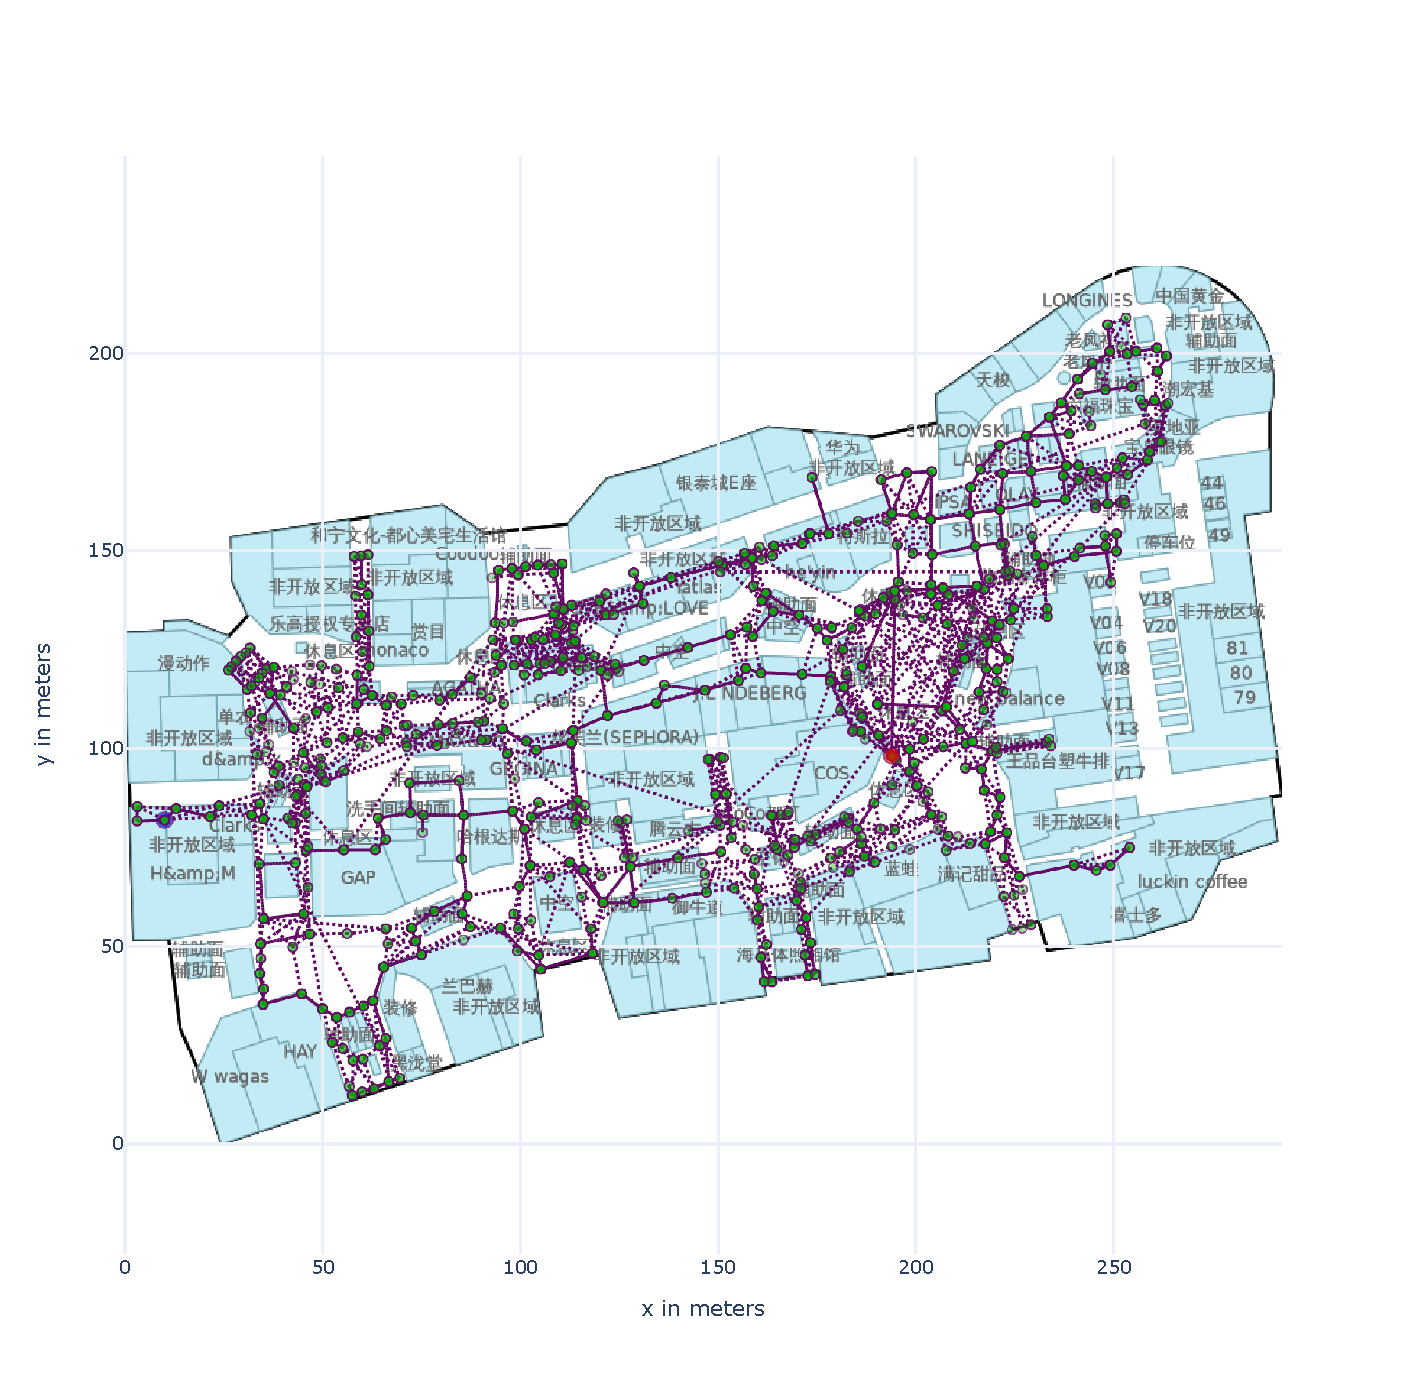
\includegraphics[scale=0.6]{images/whole_floor_visualization_wo_interpolated.pdf}
    \caption{Visualization of the 2,027 waypoints of the site Yintai City (Chengxi Branch) on floor F1}
    \label{fig:vis-wo-interpolated}
\end{figure}

Further human movement between \texttt{TYPE\_WAYPOINT} and \texttt{TYPE\_WIFI} data points may have occurred.
Therefore, a combination of the data points to directly get a location for the \ac{wifi} data points will not work, because the waypoint may have changed in that time.
Nevertheless, they can be combined using linear interpolation.

Therefore, I perform an interpolation of \texttt{TYPE\_WAYPOINT} data for \texttt{TYPE\_WIFI} timestamps in order to get a location for the \ac{wifi}.
With this interpolation, a combination of \texttt{TYPE\_WAYPOINT} and \texttt{TYPE\_WIFI} data can be done, and more data could be used for the prediction.
The interpolation results in 6549 waypoints, three times more than the original waypoints, as seen in \Cref{fig:vis-interpolated}.

\begin{figure}[h!]
    \centering
    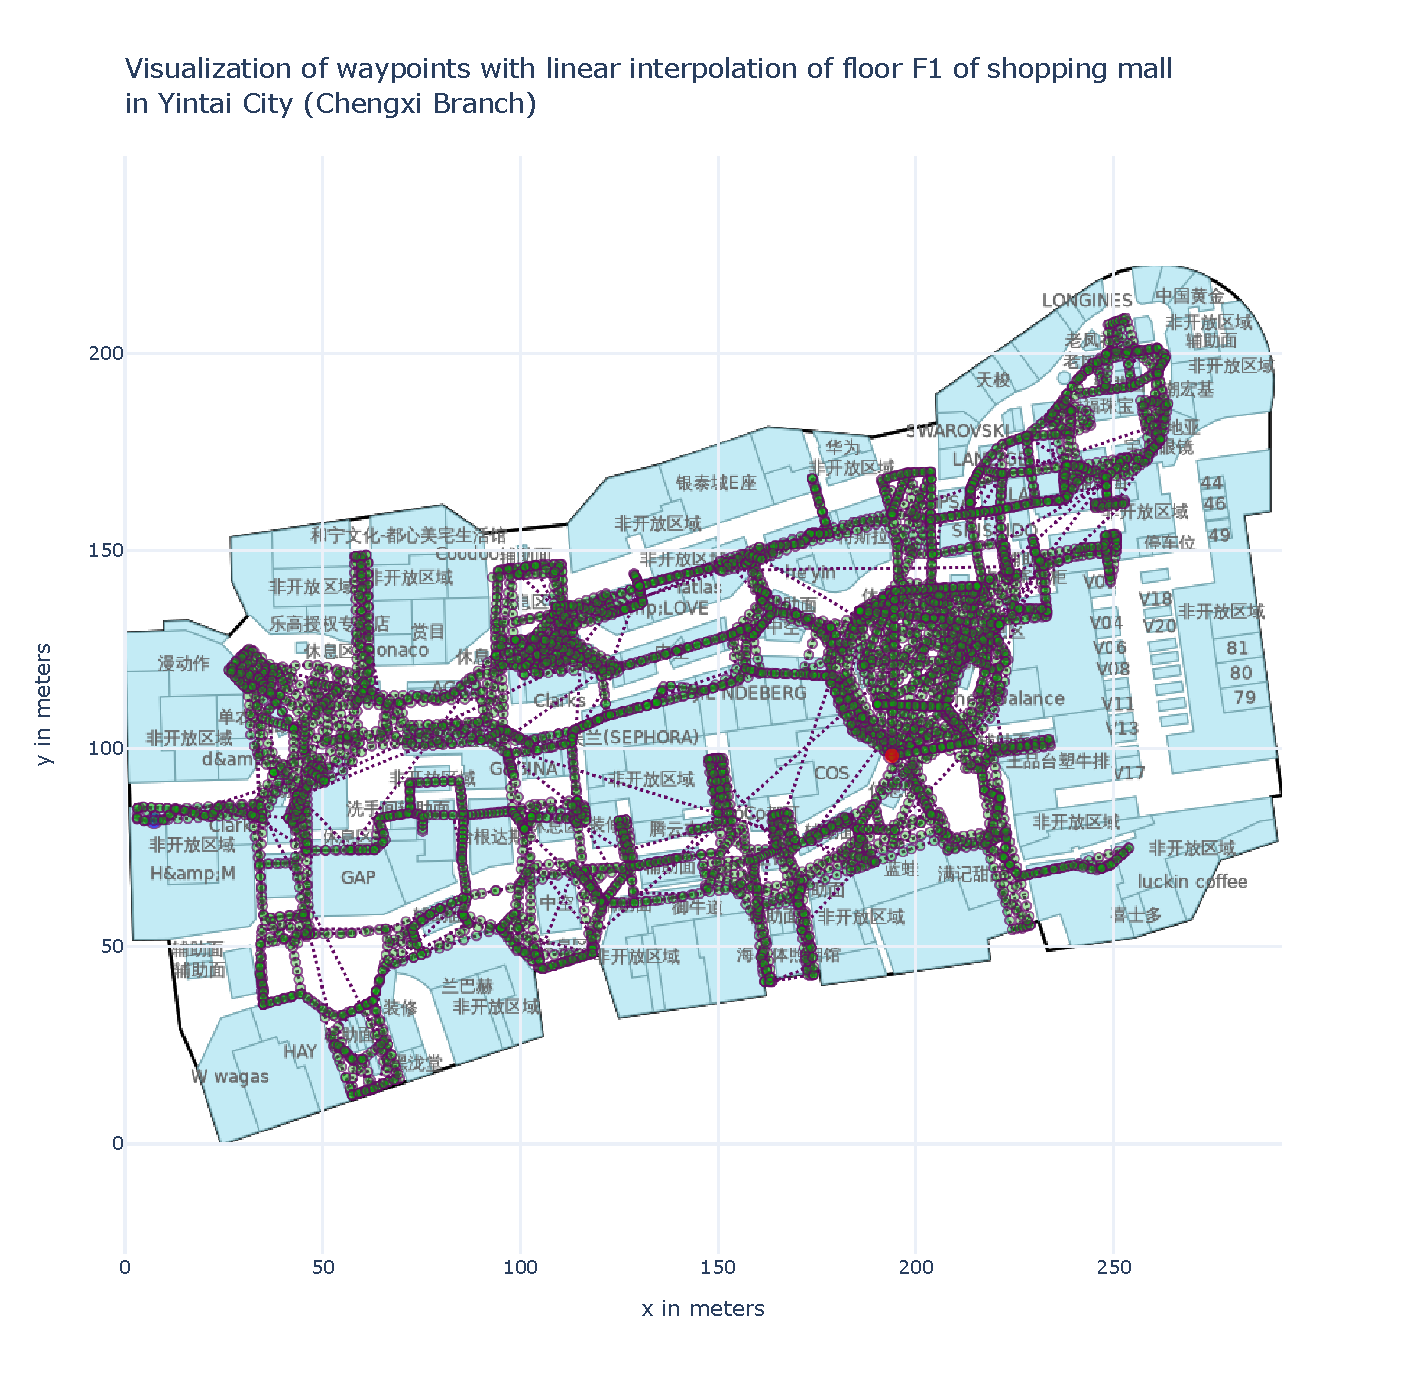
\includegraphics[scale=0.6]{images/whole_floor_visualization_interpolated.pdf}
    \caption{Visualization of the interpolated waypoints for site Yintai City (Chengxi Branch) on floor F1}
    \label{fig:vis-interpolated}
\end{figure}

As the \texttt{TYPE\_WAYPOINT} data may have changed, also the \texttt{TYPE\_ACCELEROMETER} data may have changed as well.
Although the \texttt{TYPE\_ACCELEROMETER} data is measured every 20 ms, the \texttt{TYPE\_WIFI} data may not completely match the \texttt{TYPE\_ACCELEROMETER} timestamps.
Therefore, an interpolation of \texttt{TYPE\_ACCELEROMETER} data for \texttt{TYPE\_WIFI} timestamps is done.
The acceleration values may not change significantly, but it may result in a more accurate prediction than without interpolation.
A multivariate time series with \texttt{TYPE\_WAYPOINT} and \texttt{TYPE\_ACCELEROMETER} data for each \texttt{TYPE\_WIFI} timestamp is generated.
This time series will be used for the machine learning model.
Further interpolation of the data, such as \texttt{TYPE\_GYROSCOPE}, is possible, but this thesis only utilizes the abovementioned data.

\subsection{Peculiarities of the data}\label{sec:special-cases}
The dataset analysis revealed some peculiarities, which are described in the following.

Different devices collect the data at different timestamps and days.
A problem for the time series is that the waypoint data were measured irregularly.
As \Cref{fig:vis-wo-interpolated} shows, some waypoints seem to be very distant from the next one, which can be detected by the dotted lines that go all across the floor.
\Cref{tab:metric-diff} shows the top 10 pairs of waypoints with the most significant metric differences, where \(174.77\) meters is the most significant difference.\\

\begin{figure}[h]
    \centering
    \caption{Top 10 pairs with the most significant metric differences of data from floor F1 of site Yintai City (Chengxi Branch)}

    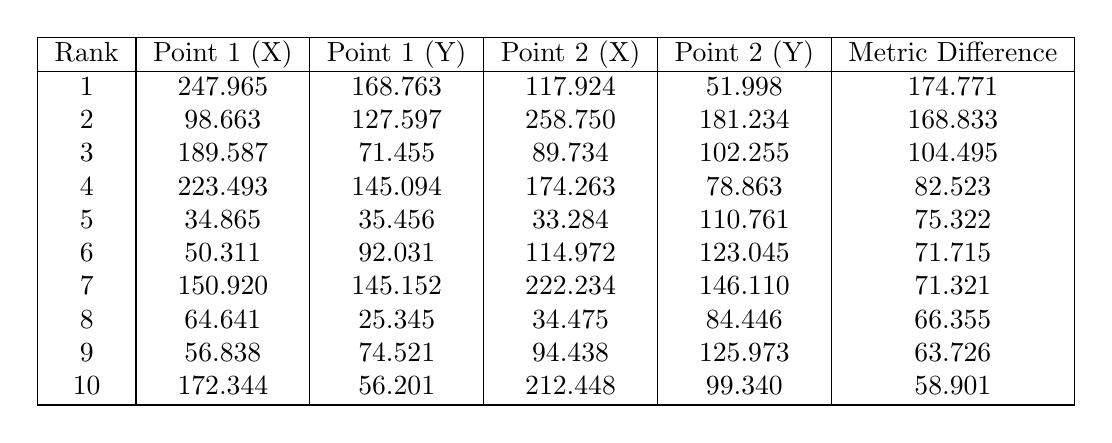
\begin{tikzpicture}
    \node (table) {
        \begin{tabular}{|c|c|c|c|c|c|}
        \hline
        Rank & Point 1 (X) & Point 1 (Y) & Point 2 (X) & Point 2 (Y) & Metric Difference \\
        \hline
        1 & 247.965 & 168.763 & 117.924 & 51.998 & 174.771 \\
        2 & 98.663 & 127.597 & 258.750 & 181.234 & 168.833 \\
        3 & 189.587 & 71.455 & 89.734 & 102.255 & 104.495 \\
        4 & 223.493 & 145.094 & 174.263 & 78.863 & 82.523 \\
        5 & 34.865 & 35.456 & 33.284 & 110.761 & 75.322 \\
        6 & 50.311 & 92.031 & 114.972 & 123.045 & 71.715 \\
        7 & 150.920 & 145.152 & 222.234 & 146.110 & 71.321 \\
        8 & 64.641 & 25.345 & 34.475 & 84.446 & 66.355 \\
        9 & 56.838 & 74.521 & 94.438 & 125.973 & 63.726 \\
        10 & 172.344 & 56.201 & 212.448 & 99.340 & 58.901 \\
        \hline
        \end{tabular}
    };
\end{tikzpicture}
    \label{tab:metric-diff}
\end{figure}

This difference is too high for a human to walk in \(1.8\) to \(2.2\) seconds, the time between two waypoints.
A human's gait speed has its maximum at about \(2.53\) meters per second \cite{bohannonComfortableMaximumWalking1997}.
So in \(2.2\) seconds, a human can walk \(5.57\) meters, which is much less than each of the values in the top 10 in \Cref{tab:metric-diff}.
Therefore, waypoints, which are more than about 5.57 meters apart, are defined as ``too apart from each other'' to walk in this time, and therefore, a split in the path will be done and generate separated files, indicating a new path.
This results in 147 files with data interpolation, which will be used for the \ac{ml} model.
However, the data in those interpolated files does not contain any information about the \ac{bssid} and corresponding \ac{rssi} values, which are needed for the prediction.
This will be solved in the following \Cref{sec:wifi-data}.


\subsection{Wi-Fi data for each timestamp}\label{sec:wifi-data}
It is evident that for a waypoint, not all \ac{rssi} values for all \acp{ap} are present because the \ac{ap} may be out of range.
In order to use the \ac{rssi} in the prediction and treat each \ac{bssid} as a class for the \ac{ml} model, an \ac{rssi} value for each \ac{ap} for each timestamp is needed.

For this, all \acp{bssid} of the site will be gathered by iterating over all \ac{wifi} data and saved in one file.
Every line contains the timestamp, and each column header is the \ac{bssid} of the \ac{ap}, and each value of the line is the \ac{rssi} value of the \ac{bssid} at the timestamp.
If an \ac{ap} is absent, a very low value \(-999\) is inserted, because the typical \ac{rssi} value ranges from \(-55\) to \(-90\) \cite{rssi_calculation}.
This ensures that it's highly improbable for an \ac{ap} to be selected for the prediction with this value.
Then, I iterate over each file with interpolated data, and for each timestamp, the \ac{bssid} and the corresponding \ac{rssi} value from the \ac{wifi} file is added to the interpolated file.
At each \texttt{TYPE\_WIFI} timestamp with waypoint and acceleration data, the \ac{rssi} value for each \ac{bssid} is now saved.
The code for this can be found in the GitHub repository in the file \texttt{preparation.ipynb}.
These files will train the \ac{ml} model.

	\chapter{Suitable Machine Learning Model}\label{ch:discuss-ml}

The floor I analyzed in \Cref{ch:data-ana} has 4795 \acp{bssid}.
Building upon the previous insights, the Yintai City (Chengxi Branch) floor 1 data has 4795 \acp{bssid}.
I will interpret each \ac{bssid} as a class, which translates to a high-dimensional classification problem with 4795 classes.
This classification task necessitates a machine learning model that can capture the underlying patterns in the data and generalize well to unseen instances.
I will discuss the classification models of \Cref{ch:background} by the following topics: Temporal Dependency Handling, Capacity and Complexity, Multivariate Data, Flexibility and Integration, and Regularization and Overfitting. 

\begin{description}
\item[Temporal Dependency Handling]
Given the goal to predict the next \ac{bssid} based on the trajectory of a user, it's imperative to select a model that can capture temporal dependencies in the data.
The irregularities in waypoint data, as mentioned in \Cref{sec:special-cases}, further emphasize the need for a model that can handle such temporal structures.
While \acp{mlp} lack this capability \cite{mlp_and_nn}, \acp{hmm} do offer some temporal structure but often fall short for longer sequences and multivariate data \cite{hmm-rabiner-1989}.
Traditional \acp{rnn} are better equipped but have their limitations, such as the vanishing gradient problem \cite{rnn_difficulties_2013}.
\acp{lstm}, in contrast, are specifically designed to handle long-term temporal dependencies, making them well-suited for our dataset with interpolated waypoints and \ac{wifi} data.
\end{description}

\begin{description}
\item[Capacity and Complexity]
Given the large number of classes (4795 \acp{bssid}), the model needs to have a considerable capacity.
\acp{mlp} can scale their capacity by adding more hidden layers and units.
They are capable of modeling complex relationships within data through their nonlinear activations.
\acp{hmm} have limitations in handling the complexity of multi-class and multivariate problems due to their inherent Markovian assumptions and discrete state representations and may struggle with such a high-dimensional problem.
Traditional \acp{rnn} suffer from the vanishing gradient problem, especially in longer sequences, which limits their ability to capture long-term dependencies effectively \cite{rnn_difficulties_2013}.
With 4,795 classes, the model needs a considerable capacity to differentiate between the subtle differences in patterns that might exist among them. 
\acp{lstm}, being deep learning models, can scale effectively in terms of capacity by adding more layers or units while still maintaining their ability to handle temporal data.
\end{description}

\begin{description}
\item [Multivariate Data]
The data at hand is multivariate, with features such as waypoint, accelerometer, and \ac{wifi} data.
While \acp{mlp} can handle multivariate data, they treat each feature and time step independently, often missing out on the interdependencies.
\acp{hmm} are primarily designed for univariate data. Extending them to multivariate scenarios requires additional complexities and assumptions.
\acp{rnn} and \acp{lstm} can seamlessly handle multivariate time series data. 
Their recurrent nature allows them to effectively process each time step with multiple features.
\end{description}

\begin{description}
\item[Flexibility and Integration]
Considering the interpolated data and the various preprocessing steps undertaken, as mentioned in \Cref{sec:prep-on-data-for-an-ml-model}, a flexible model that can be integrated with other architectures or preprocessing steps is desirable. 
\acp{mlp} are very flexible and can generally be used to learn a mapping from inputs to outputs. \cite{mlp-vs-cnn-vs-rnn} 
As I want to learn, which BSSID is the next one, this may be a good fit.
\acp{hmm} are primarily designed for capturing state transitions in sequential data and may not be suitable for tasks requiring the integration of spatial and temporal information.
Their rigid assumptions about state transitions limit their flexibility in capturing complex patterns \cite{hmm-rabiner-1989}.
Traditional \acp{rnn} can capture short-term dependencies and are relatively simpler to integrate with other architectures due to their sequential nature.
Also, \acp{lstm} can easily be integrated to capture both temporal and spatial features. 
This flexibility of \acp{rnn} and \acp{lstm} is advantageous when dealing with complex and varied data sources.
\end{description}

\begin{description}
\item[Regularization and Overfitting]
Given the large number of data points, as detailed in \Cref{tab:data_summary}, and the intricate relationships between them, the potential for overfitting is high.
Therefore, dropouts may be used to prevent overfitting for each model \cite{srivastava14a}.
While \acp{rnn} might be more prone to overfitting \cite{rnn_difficulties_2013}, \acp{mlp}, \acp{hmm}, and \acp{lstm} offer better regularization capabilities.
\end{description}

\begin{table}[h]
    \centering
    \caption{Suitability of models for various requirements.}
    \begin{tabular}{l|c|c|c|c}
        & MLP & HMM & RNN & LSTM \\
        \hline
        Temporal Dependencies & & \checkmark & \checkmark & \checkmark \\
        Capacity & \checkmark & & & \checkmark \\
        Multivariate Data & & & \checkmark & \checkmark \\
        Flexibility & \checkmark & & \checkmark & \checkmark \\
        Overfitting & \checkmark & \checkmark & & \checkmark \\
    \end{tabular}
    \label{tab:model_suitability}
\end{table}


In conclusion, while \acp{mlp}, \acp{hmm}, and traditional RNNs have their strengths and have been successful in many applications, they have problems with multivariate time series classification with many classes.
The classification problem for this thesis demands a model that can efficiently capture temporal patterns, scale in capacity, and handle multivariate data.
As \Cref{tab:model_suitability} shows, \acp{lstm} can deal with this challenge due to their unique architecture and properties, making them the preferred choice for this task and the selected model for our implementation.

	\include{content/data_preperation}
	\chapter{Implementation}\label{sec:implementation}

All the code for this implementation can be found in the GitHub repository \cite{github-repo}.

\section{Preprocessing}
\begin{itemize}
    \item Preprocessing with numpy and pandas
    \item Use data from \cref{sec:data-ana} for preprocessing
    \item Load data from files of floor with most files
    \item Create a target variable (based on RSSIs of BSSIDs)
    \item Normalize the data.
    \item Create sequences of data based on window\_size variable.
    \item Encode the target variable, which is a variable with 4795, where 1 means the class is the nearest \ac{ap} and 0 means the class is not the nearest \ac{ap}, which results in a one-hot encoding.
    \item Split the data into training and testing set. (80/20)
\end{itemize}

% \begin{figure}[h!]
%     \centering
%     
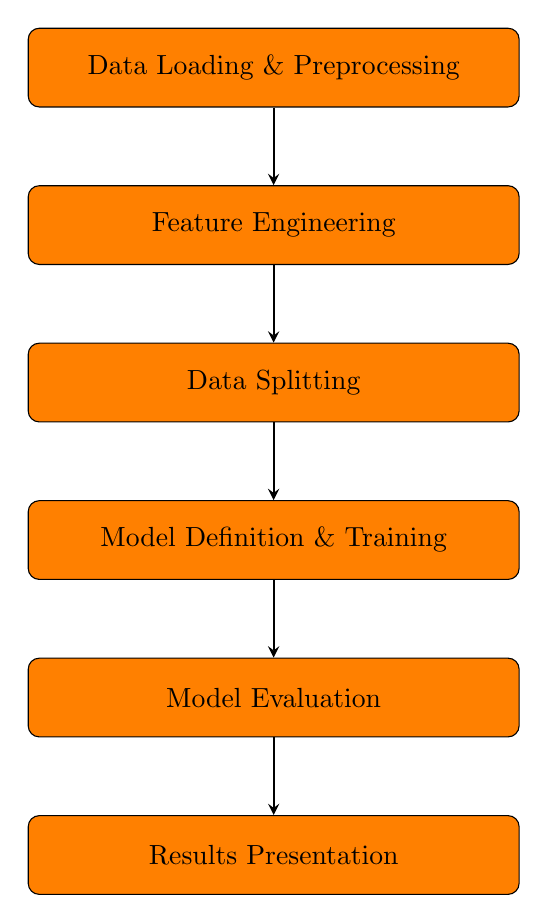
\begin{tikzpicture}
    % Define the styles for the processes and arrows
    \tikzstyle{process}=[rectangle, rounded corners, draw=black, fill=orange, text centered, text width=6cm, minimum height=1cm]
    \tikzstyle{arrow}=[thick,->,>=stealth]

    % Draw the processes
    \node[process] (data_loading) at (0, 0) {Data Loading \& Preprocessing};
    \node[process] (feature_engineering) at (0, -2) {Feature Engineering};
    \node[process] (data_splitting) at (0, -4) {Data Splitting};
    \node[process] (model_definition) at (0, -6) {Model Definition \& Training};
    \node[process] (model_evaluation) at (0, -8) {Model Evaluation};
    \node[process] (results_presentation) at (0, -10) {Results Presentation};

    % Draw the arrows between the processes
    \draw[arrow] (data_loading) -- (feature_engineering);
    \draw[arrow] (feature_engineering) -- (data_splitting);
    \draw[arrow] (data_splitting) -- (model_definition);
    \draw[arrow] (model_definition) -- (model_evaluation);
    \draw[arrow] (model_evaluation) -- (results_presentation);
\end{tikzpicture}

%     \caption{Flow diagram of the implementation process.}
%     \label{fig:flow_diagram}
% \end{figure} 

\section{\ac{lstm} Training and Testing}
\begin{itemize}
    \item Use Keras library for implementation \cite{keras}
    \item Model: LSTM layer, Dense layer with softmax activation
    \subitem Sequences are of length window\_size for each entry in the dataset
    \subitem Inputs are (window\_size, number\_of\_features (which are 6 + number of BSSIDs)), see \cref{fig:lstm_architecture}
    \item Generate predictions on the test set
    \item Get class with the highest probability as prediction
    \item Get top 3 predictions for the test set and check if the target variable is in the top 3 predictions.
\end{itemize}

\begin{figure}[h!]
    \centering
    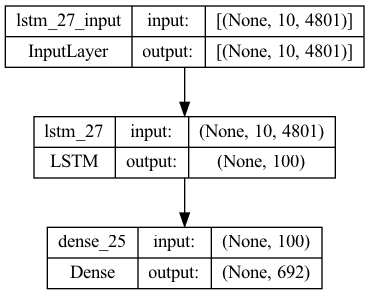
\includegraphics[scale=0.5]{images/model_plot.png}
    \caption{An example LSTM Network with Input, LSTM and Dense Layer with 4801 Features and window\_size of 10.}
    \label{fig:lstm_architecture}
\end{figure}

\section{Tuning model and hyperparameters}
\begin{itemize}
    \item try out different hyperparameters also in combination
    \subitem Number of units in the LSTM layer = \{100, 150, 200, 350, 500, 1000, 2000\}
    \subitem batch size = \{16, 32, 64\}
    \subitem window size = \{3, 5, 10, 20\}
\end{itemize}

%\noindent

	\chapter{Evaluation}\label{ch:evaluation}

For the evaluation of the model, I do the following:
First, the predictions of the test set are in \texttt{X\_test}.
Since the predictions are probabilities for each class, a conversion of the highest probability as true labels in \texttt{y\_test} is done because this value will be the predicted \ac{ap}.
Those are one-hot encoded, as described in \Cref{ch:implementation}.
Then, I decode the one-hot encoded classes to the original classes, which can be done by \texttt{inverse\_transform} with the encoder.

Finally, I select the target value of the predictions and compare it with the corresponding true label for the timestamp.
If they are equal, the prediction is correct, otherwise it is false.
The \threeAP prediction accuracy of the \ac{lstm} model, so that one of the three predicted \ac{bssid} is the one with the highest \ac{rssi} value, is 76\,\%.
The predictions ranging from a set size of one to five are also evaluated, as shown in \Cref{fig:comparison_ml_heuristic_1_to_5}.

\begin{figure}[h]
    \centering
    \includegraphics*[scale=0.53]{images/comparison_ml_heuristic_1_to_5.pdf}
    \caption{Comparison of the Probabilities of correctly predicting the set size of one to five \acp{ap} in the ML Model and the Heuristic Approach.}
    \label{fig:comparison_ml_heuristic_1_to_5}
\end{figure}

Instead of predicting \threeAP, a heuristic approach could be used and will be compared with the model in the following.
The heuristic chooses the latest \ac{ap} with the highest signal strength as following \ac{ap}.
If it is not the following highest \ac{rssi}, it will proceed with the latest second highest until the fifth highest to compare it to our approach. %\fmhkn{versteh ich nicht... ? was beduet dieser Satz? }
\Cref{fig:comparison_ml_heuristic_1_to_5} shows the accuracy of this heuristic approach for choosing the latest highest to the fifth highest \ac{ap}.

For predicting the set size of one, so the predicted \ac{ap} is correct, the heuristic's accuracy outperforms the \ac{ml} model by 3.5\,\%.
For the set size of two, the \ac{ml} model outperforms the heuristic by 0.3\,\%.
For \threeAP the prediction accuracy improves by 1.7\,\% compared to the heuristic approach.
Four and five set sizes outperform the heuristic by 2.2\,\%, and 1.2\,\%, respectively.

Regarding the execution time, the \ac{ml} model needs nearly 12 hours to tune.
The training of the proposed \ac{lstm} model takes about 25 minutes for a five-fold cross-validation.
The heuristic approach must only choose the three highest \ac{rssi} values out of 4795, which is much faster.
The heuristic is much easier to implement and execute than the \ac{ml} model.

The \ac{ml} model needs to be trained for each floor of a mall separately, as the \ac{ap} are different on each floor.
The heuristic approach can be used for all floors, as it only needs the latest \ac{rssi} values of the \acp{ap}.

One of the significant strengths of the machine learning model is that it utilizes user trajectories.
However, the heuristic is a simpler and faster approach for predicting the following \ac{ap}.
This approach can capture complex patterns and relationships that other models might overlook.
However, there are also inherent weaknesses.
The model has to deal with 4795 classes, and given that it only relies on six features, this may compromise its predictive accuracy.
This limitation might result in the model predicting worse than initially expected.

	\chapter{Conclusion}\label{ch:conclusion}
 
\ac{ap} prediction with user movement is a hard task with many classes.
Although \ac{lstm} is the best choice among the discussed models for this task, the prediction accuracy for selecting on of the top 3 \acp{ap} is XX\%.
In the future, the model could also be trained for other floors and sites, which would likely result in similar accuracies.

With fewer classes, the \ac{lstm} model could predict better, which could be a reason why \ac{ml} model prediction is only slightly better than the simpler heuristic approach.
Furthermore, the model could be enhanced with other sensor data such as gyroscope and magnetic field data.
Maybe the sliding window size is too small, and a larger window size could improve the prediction.
Also, one could generate data from mobile devices or \acp{ap}, so that more information such as location of the \ac{ap} and setup is known and can be used in prediction.

%\noindent


	% Bibliographie
	\ifisbook\cleardoubleemptypage\fi
	\phantomsection\addcontentsline{toc}{chapter}{\refname}
	\printbibliography[category=cited]
	
	% ggf. Anhang
	\appendix\chapter{\appendixname}

\section*{Eins (ohne extra Eintrag im Inhaltsverzeichnis)}
Lorem ipsum dolor sit amet, consetetur sadipscing elitr, sed diam nonumy eirmod tempor invidunt ut labore et dolore magna aliquyam erat, sed diam voluptua. At vero eos et accusam et justo duo dolores et ea rebum.
 % example
	
	% ggf. bei englischen Arbeiten den deutschen Abstract nach hinten verschieben
	\ifisbook\pagestyle{plain}\cleardoubleemptypage% => Wenn die Arbeit auf Englisch verfasst wurde, verlangt das Studienreferat einen englischen UND deutschen Abstract (der dt. Abstract kann dann ggf. auch ans Ende der Arbeit)

% deutsche Zusammenfassung
\null\vfil
\begin{otherlanguage}{ngerman}
\begin{center}\textsf{\textbf{\abstractname}}\end{center}

\noindent ...

\end{otherlanguage}
\vfil\null



\fi

	% Eigenständigkeitserklärung
	\ifisbook\pagestyle{plain}\cleardoubleemptypage% => Laut Aussage des Studienreferats braucht es - auch wenn die Arbeit in englischer Sprache verfasst ist - KEINE separate Version der Eigenständigkeitserklärung auf Englisch. Sowohl für Arbeiten in deutscher Sprache als auch für Arbeiten in englischer Sprache genügt EINE EINZIGE Eigenständigkeitserklärung auf DEUTSCH.
\begin{otherlanguage}{ngerman}

\begin{center}\textsf{\textbf{Eidesstattliche Erklärung}}\end{center}
Hiermit versichere ich, dass meine {\hpitype} \enquote{\hpititle} selbstständig verfasst wurde und dass keine anderen Quellen und Hilfsmittel als die angegebenen benutzt wurden. Diese Aussage trifft auch für alle Implementierungen und Dokumentationen im Rahmen dieses Projektes zu.\\

\noindent
Potsdam, den 11. September 2023,
\vspace{2cm}

\begin{center}
\begin{tabular}{C{6cm}}
\hline
{\small({\hpiauthor})}
\end{tabular}
\end{center}

\end{otherlanguage}


\fi

\end{document}